The considerable disadvantage of nine-noded biquadratic Lagrange elements compared to
a bilinear element is the increased number of degrees of freedom. Especially both degrees of
freedom of the middle node are increasing the linear equation system of the assembled system
which has to be solved by two equations per discrete Lagrange element. On the other hand, the
same middle node is not necessary for preservation of compatibility with the adjacent element.

This means that the number of degrees of freedom can especially be reduced at system level
by utilization of serendipity elements instead of Lagrange elements. Hence, the motivation for
generation of quadratic serendipity elements with no middle node is given.

In the sections that follow we will discuss shape functions, approximation of geometry and of
the displacement field. Since the development of the differential operator and of element matrices
and vectors has to be accomplished in analogy with the four-noded or nine-noded Lagrange
element, the presentation of this procedure is abandoned.
\begin{figure}[H]
    \centering
    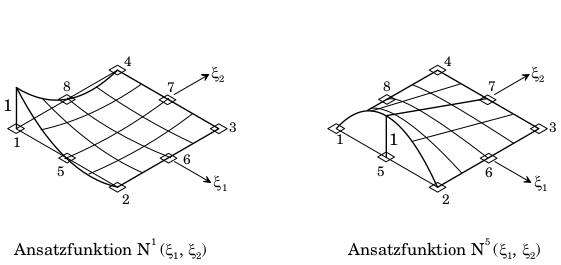
\includegraphics[scale=0.6]{Figure2/Chap2/shpaefunctionq8.png}
    \caption{Generation of biquadratic serendipity shape functions}
    \label{fig:my_label}
\end{figure}

\subsection{Shape Functions}
Contrary to a biquadratic \textsc{Lagrange} element, the shape functions of the eight-noded serendipity element cannot be generated from one-dimensional Lagrange interpolation functions. They
are constructed directly by means of the demands on shape function $N^i(\xi)$ to take on the value
one at node $i$ and the value zero at node $j \ne i$ . The generation of principally different shape functions of corner nodes and side middle nodes is shown in figure {\ref{fig:my_label}.
Here, as an example we have developed the shape functions of corner node one and side middle node eight.

The terms in $\xi_ 1$ and $\xi_ 2 $ appearing in shape functions $ N^ 1 , N^ 5$ and $N^ 8$ are designated by $p = 2$
in the Pascal triangle in figure \ref{fig:3.6}. The remaining shape functions of a quadratic serendipity element are written without deriving.
\begin{equation}
 \begin{aligned} N^{1}(\boldsymbol{\xi}) &=-\frac{1}{4}\left(1-\xi_{1}\right)\left(1-\xi_{2}\right)\left(1+\xi_{1}+\xi_{2}\right) & \qquad N^{5}(\boldsymbol{\xi}) &=\frac{1}{2}\left(1-\xi_{1}^{2}\right)\left(1-\xi_{2}\right) \\ N^{2}(\boldsymbol{\xi}) &=-\frac{1}{4}\left(1+\xi_{1}\right)\left(1-\xi_{2}\right)\left(1-\xi_{1}+\xi_{2}\right) & N^{6}(\boldsymbol{\xi}) &=\frac{1}{2}\left(1+\xi_{1}\right)\left(1-\xi_{2}^{2}\right) \\ N^{3}(\boldsymbol{\xi}) &=-\frac{1}{4}\left(1+\xi_{1}\right)\left(1+\xi_{2}\right)\left(1-\xi_{1}-\xi_{2}\right) & N^{7}(\boldsymbol{\xi}) &=\frac{1}{2}\left(1-\xi_{1}^{2}\right)\left(1+\xi_{2}\right) \\ N^{4}(\boldsymbol{\xi}) &=-\frac{1}{4}\left(1-\xi_{1}\right)\left(1+\xi_{2}\right)\left(1+\xi_{1}-\xi_{2}\right) & N^{8}(\boldsymbol{\xi}) &=\frac{1}{2}\left(1-\xi_{1}\right)\left(1-\xi_{2}^{2}\right) \end{aligned} 
\end{equation}
\subsection{Geometry}
The element coordinate vector X e has a dimension reduced by two as opposed to the vector $X^e$
of a Lagrange element, which corresponds to the coordinates of the middle node.
\begin{equation}
 \boldsymbol{X}^{e}=\left[\begin{array}{llllllll}\boldsymbol{X}^{e 1T} & \boldsymbol{X}^{e 2 T} & \boldsymbol{X}^{e 3 T} & \boldsymbol{X}^{e 4 T} & \boldsymbol{X}^{e 5 T} & \boldsymbol{X}^{\epsilon 6 T} & \boldsymbol{X}^{e 7 T} & \boldsymbol{X}^{e 8 T}\end{array}\right]^{T} 
 \label{eqn:3.151} 
\end{equation}

Geometry of a serendipity element is usually described as function of natural coordinates $\xi$
according to equation (\ref{eqn:3.42}) with the shape functions matrix
\begin{equation}
 \mathbf{N}^{i}(\boldsymbol{\xi})=\left[\begin{array}{cc}N^{i}(\boldsymbol{\xi}) & 0 \\ 0 & N^{i}(\boldsymbol{\xi})\end{array}\right] \quad \mathbf{N}(\boldsymbol{\xi})=\left[\begin{array}{ccccc}\mathbf{N}^{1} & \mathbf{N}^{2} & \cdots & \mathbf{N}^{7} & \mathbf{N}^{8}\end{array}\right] 
 \label{eqn:3.152} 
\end{equation}

%--------------------------------------------
\subsection{Jacobi Transformation}
The \textsc{Jacobi} matrix $J(\xi)$, that is the inverse Jacobi matrix necessary to generate the derivatives with respect to physical coordinates by means of derivatives with respect to natural coordinates,
can be computed in analogy according to equations (\ref{eqn:3.46}) that is (\ref{eqn:3.48}) or
(\ref{eqn:3.52}).
\begin{equation}
 \frac{\partial X_{\beta}(\boldsymbol{\xi})}{\partial \xi_{\alpha}}=\sum_{i=1}^{N N} X_{\beta}^{e i} N_{; \alpha}^{i}(\boldsymbol{\xi}) \qquad \qquad \frac{\partial \boldsymbol{X}(\boldsymbol{\xi})}{\partial \xi_{\alpha}}=\boldsymbol{X}_{; \alpha}(\boldsymbol{\xi})=\mathbf{N}_{; \alpha}(\boldsymbol{\xi}) \boldsymbol{X}^{e} 
 \label{eqn:3.143} 
\end{equation}

Transformation of a differential surface element $dA$ follows according to equation (\ref{eqn:3.58}) with the help of the Jacobi determinant.
%----------------------------------------
\subsection{Approximation of element quantities}

Element quantities, displacements, accelerations and variation of displacements are approxi-
mated in analogy with the Lagrange element.
\begin{equation}
 \begin{aligned} \boldsymbol{u}(\boldsymbol{\xi}) & \approx \tilde{\boldsymbol{u}}(\boldsymbol{\xi})=\mathbf{N}(\boldsymbol{\xi})  \boldsymbol{u}^{e} & \boldsymbol{u}^{e} &=\left[\begin{array}{lllll}u_{1}^{e 1} & u_{2}^{e 1} & \cdots & u_{1}^{e 8} & u_{2}^{e 8}\end{array}\right]^{T} \\ 
 \delta \boldsymbol{u}(\boldsymbol{\xi}) & \approx \delta \tilde{\boldsymbol{u}}(\boldsymbol{\xi})=\mathbf{N}(\boldsymbol{\xi}) \delta \boldsymbol{u}^{e} & \delta \boldsymbol{u}^{e}&=\left[ 
 \begin{array}{lllll}
 \delta u_{1}^{e 1} &\delta u_{2}^{e 1}& \cdots &\delta u_{1}^{e 8}& \delta u_{2}^{e 8}
 \end{array}
 \right]^{T} \\ 
 \ddot{\boldsymbol{u}}(\boldsymbol{\xi}) & \approx \tilde{\tilde{u}}(\boldsymbol{\xi})=\mathbf{N}(\boldsymbol{\xi}) \ddot{u}^{e} & \ddot{\boldsymbol{u}}^{e}&=\left[\begin{array}{lllll}\ddot{u}_{1}^{e 1} & \ddot{u}_{2}^{e 1} & \cdots & \ddot{u}_{1}^{e 8} & \ddot{u}_{2}^{e 8}\end{array}\right]^{T} \end{aligned} 
\end{equation}

The dimension of the element vector is by two smaller than that of an element with a middle
node. Element vectors $u _e$ , $\varepsilon u^e $and $\ddot{u}^ e$ are of dimension $16 × 1$ and the shape function matrix
$\boldsymbol{N}$ is of dimension $2 \times 16$.

